\section{Results}
\label{sec-results}
To evaluate RSR we use a generic implementation of A* and discuss performance 
in terms of search time speedup. That is, the relative improvement to the average 
time A* needs to solve an instance when running on a pruned  vs. unpruned grid.
For example, a speedup of 2.0 is twice as fast (higher is better).
%
%while
%a node expansion speedup of 2.0 indicates half the number of nodes were expanded.
%In each case higher is better.
Note that on approximately 2\% of all instances the start and goal are located
in the same rectangle and RSR computes the optimal solution without
search.  We exclude these instances from our results on the basis that they are 
outliers, even though RSR solves them in constant time.

\par 
\begin{figure}[t]
       \begin{center}
				   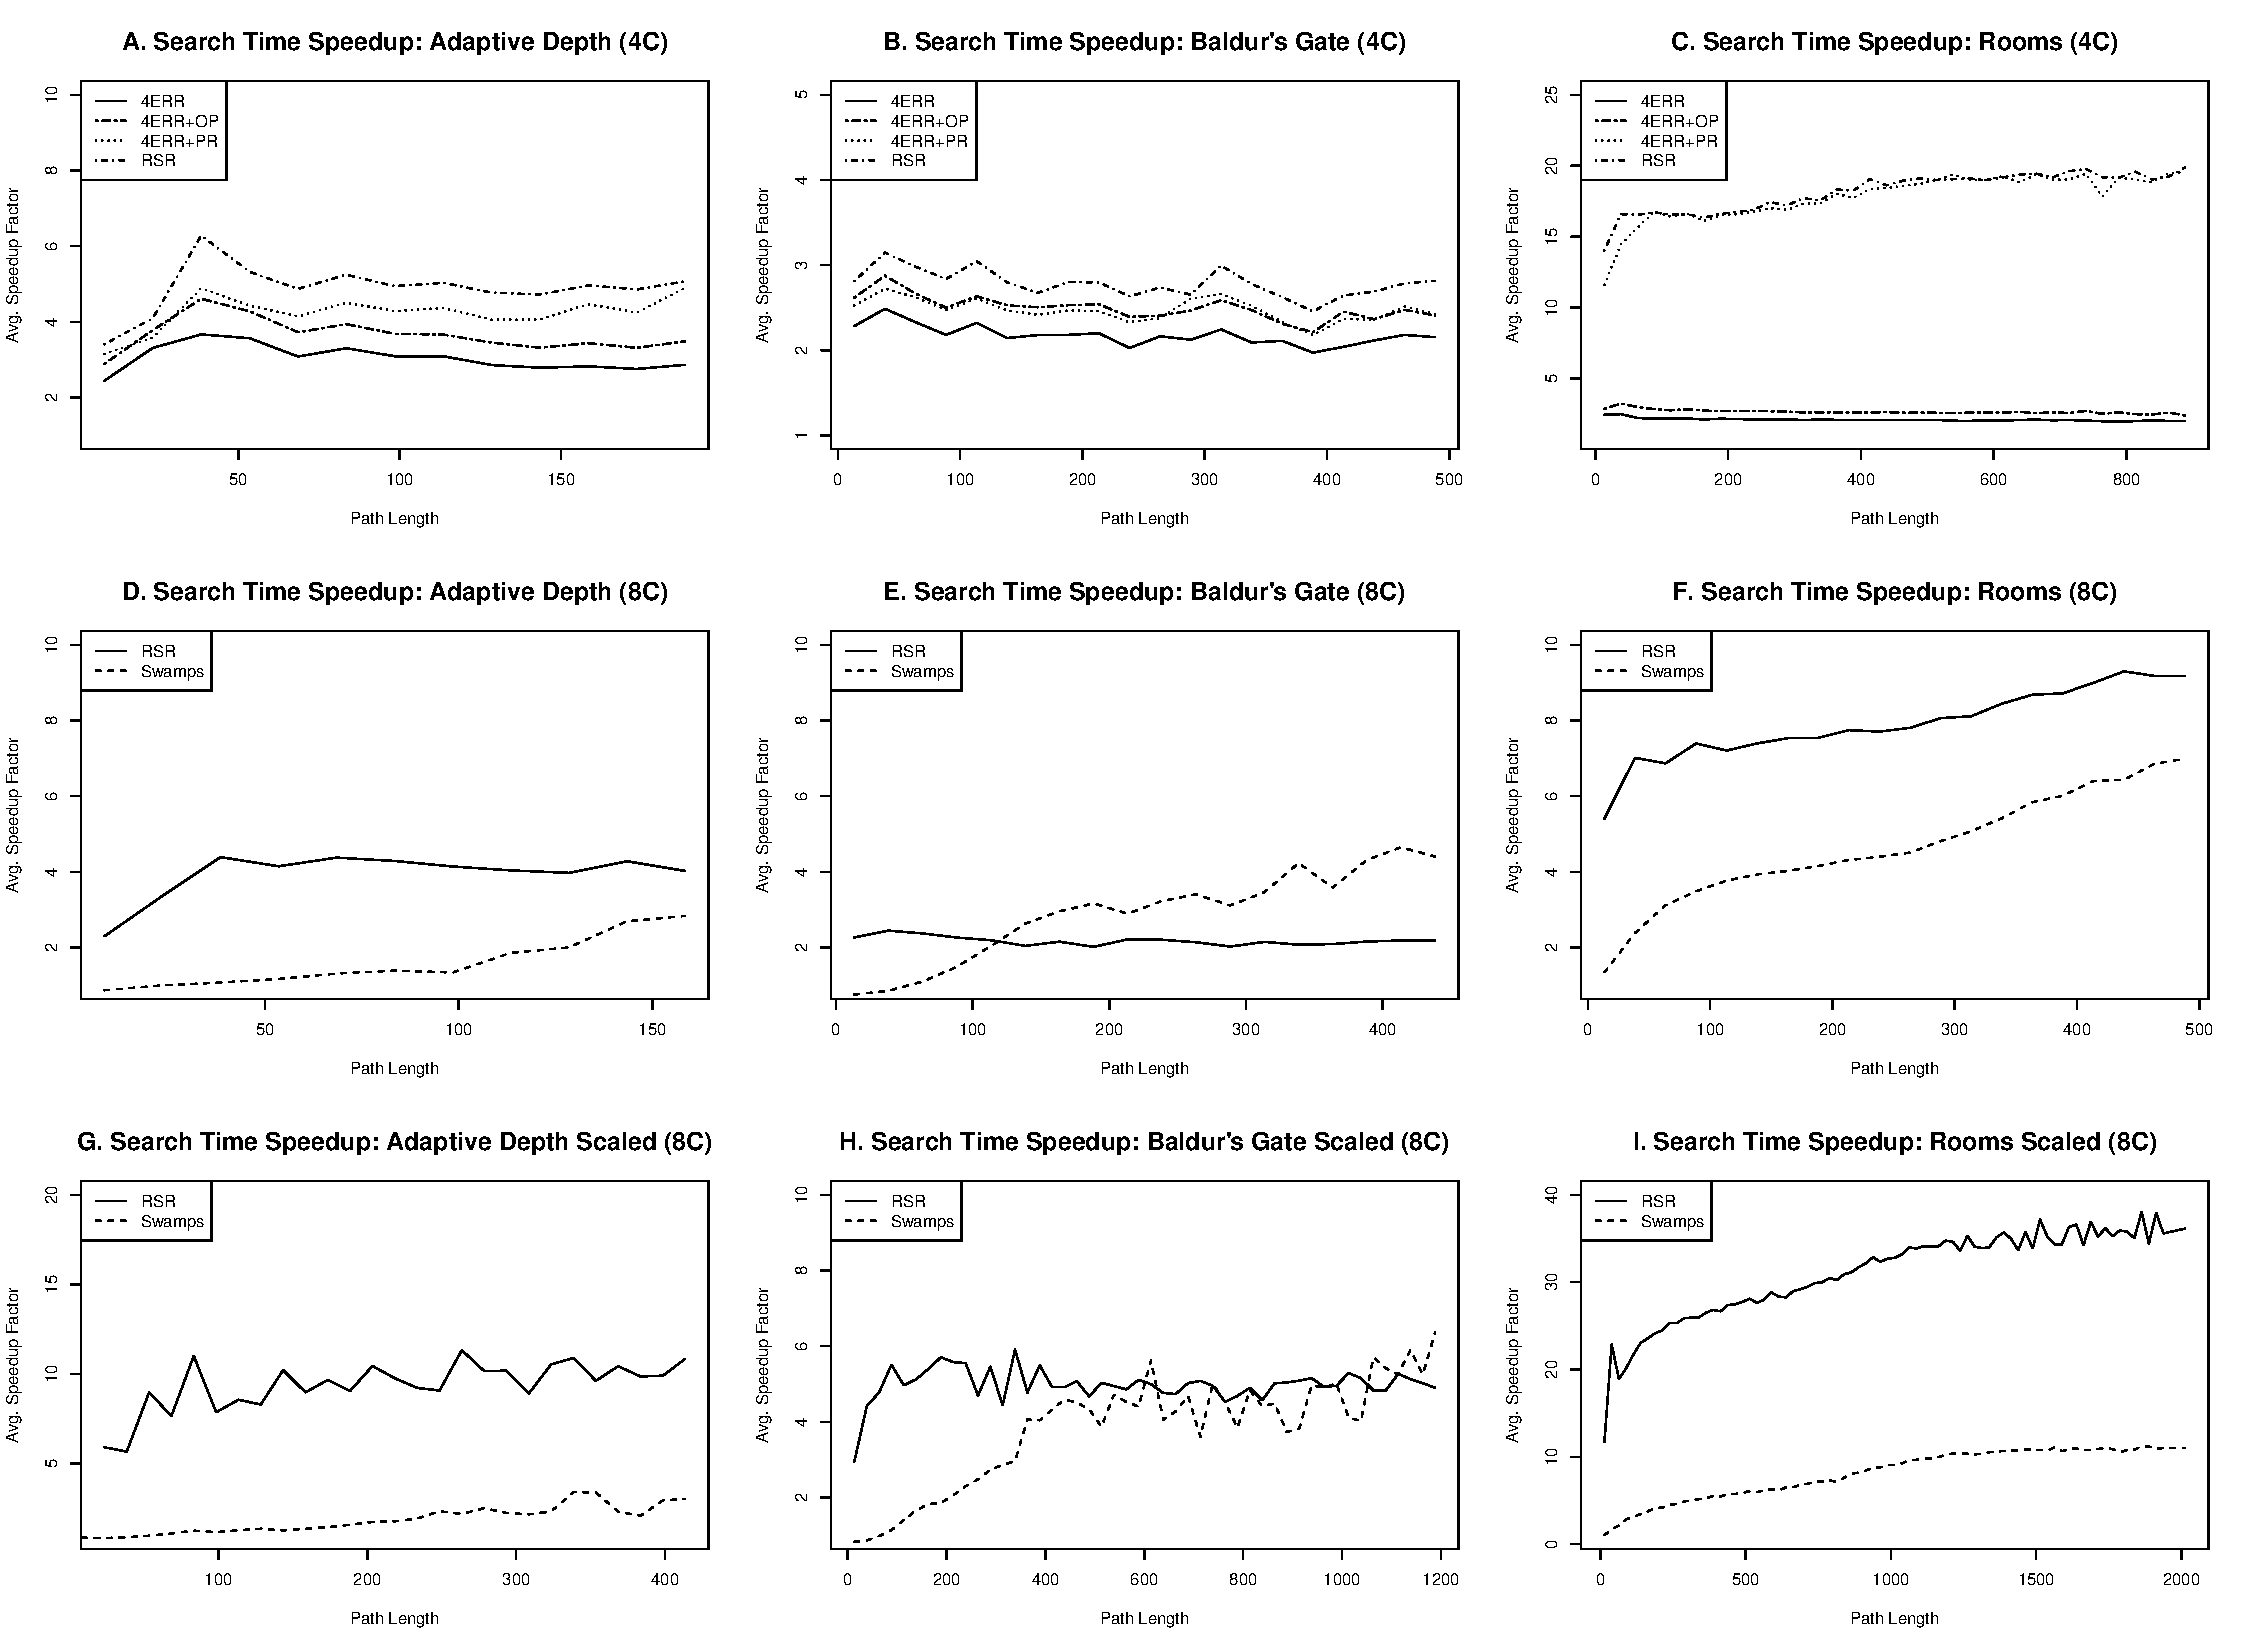
\includegraphics[width=0.97\columnwidth, trim = 10mm 10mm 10mm 0mm]{diagrams/speedup.pdf}
       \end{center}
       \caption{Average A* speedup on each of our three benchmarks. 
		Results are given in terms of relative improvement to A* search time (i.e. speedup).}
\label{fig-speedup}
\end{figure}


\textbf{Pre-processing Times: } 
RSR takes very little time to pre-process all input maps. 
We did not encounter any map that took longer than a second; most required 
half a second or less.
Thus RSR appears well suited to
pathfinding in dynamic environments as outlined in Section \ref{sec:memory}.

\textbf{Comparison to 4ERR: }
We now compare the performance RSR against the 4ERR~\cite{harabor10} graph
pruning algorithm. Here we restrict our attention to 4-connected maps.  To
assess the individual impact of both perimeter reduction (PR) and online node
pruning (OP) we also develop and compare two variant algorithms: 4ERR+PR and
4ERR+OP. 
\par
Figure \ref{fig-speedup} (A to C) presents our main result. RSR dominates
convincingly across all instances allowing us to conclude it is the better
choice on 4-connected maps. 
Of the variants, 4ERR+PR yields the biggest improvement, speeding up A* by up to 20 times.
4ERR+OP compares well on Adaptive Depth and Baldur's Gate but is of little benefit on 
Rooms where perimeter pruning has already reduced the branching factor.
\par
\textbf{Comparison to Swamps:}
Next, we RSR with Swamps-based pruning~\cite{pochter10}.  
We used the authors' source code, including their own implementation of A*, and 
ran all experiments using their recommended parameters: a swamp seed radius of 6 
and ``no change limit'' of 2. Figure \ref{fig-speedup} (D to F) gives the main
result on the 8-connected variants of our three benchmarks.
On Adaptive Depth and Rooms, where the terrain can be naturally decomposed into
rectangles, RSR achieves higher speedups and is shown consistently better than Swamps. 
On Baldur's Gate, where this is not the case, Swamps-based pruning is more
effective. 
\par
To measure the effect that larger open areas have on search time, we scaled
every map in each benchmark by a factor of 3. We then generated a new set of 100
problem instances per map. Figure \ref{fig-speedup} (G
to I) show the results.  
The overall gain for Swamps is very small while RSR show dramatic improvement.
This is not surprising: Swamps prune out
areas that can be avoided without detour while symmetry reduction allows
faster exploration of areas to be searched.
Since the two ideas are orthogonal, a natural extension would be to combine them: 
first, apply symmetry reduction to a grid; then, apply a Swamps-based 
decomposition to the resultant graph.

\input table_portals

\textbf{Comparison to Portal Heuristic:}
Table 2 compares RSR against published results for the enhanced variant of the
recent Portal Heuristic algorithm~\cite{goldenberg10}.  As in that work we focus
on 4-connected variants of Baldur's Gate and Rooms.
\par
PH-e performs well when it can decompose the map into areas of similar size with
few transitionary nodes connecting them.
RSR performs well when it can decompose the map into large rectangles with few
perimeter nodes.
On Rooms, both decomposition approaches are highly effective. 
On Baldur's Gate both are comparatively less effective.
Notice however that PH-e requires up to 7 times more memory than RSR to achieve
similar results.
As with Swamps, we believe PH-e is entirely orthogonal to RSR and the two can be 
easily combined. For example, PH-e could be used to more accurately guide search
on a map pruned by RSR. Alternatively, symmetry elimination could be used to 
speed up pathfinding between successive pairs of portals during PH-e's refinement phase.

